\section{Аналитический раздел}
\subsection{Кубик Рубика}
Кубик Рубика (в честь Эрнё Рубика) --- механическая головоломка, представляющая из себя куб,
каждая грань которого имеет уникальный цвет и делится малыми кубами на 9 частей (26 в сумме со всех сторон) \cite{bib:how_to_assemble}.
Механизм, располагающийся в центре кубика, позволяет вращать каждую грань относительно кубика Рубика.
Таким образом, набор случайных поворотов граней приводит к «разборке» кубика рубика.
Обратная «сборка» заключается в последовательности поворотов грани так,
чтобы каждая грань кубика рубика снова стала одноцветной.

\begin{figure}[ht]
	\centering
	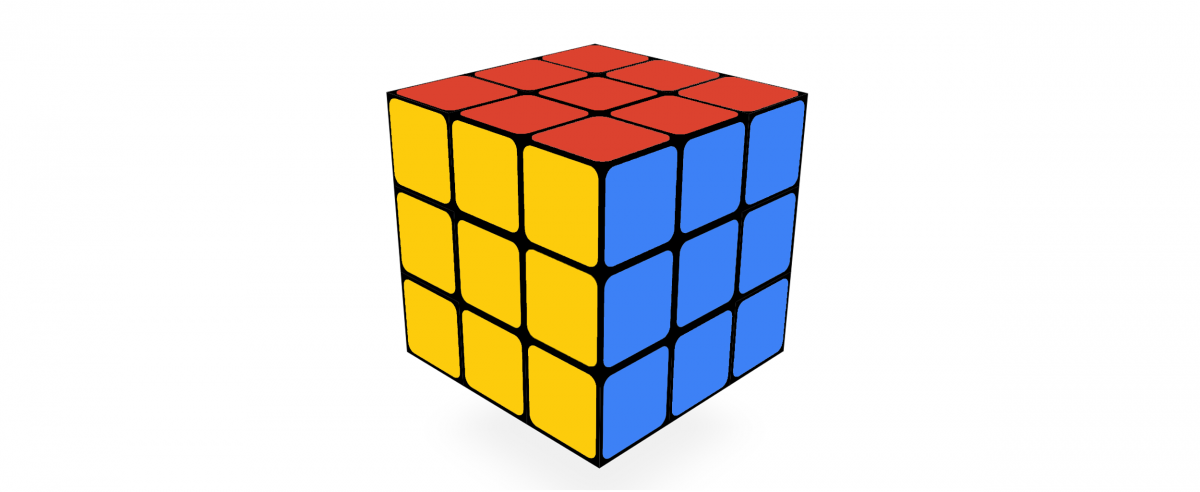
\includegraphics[width=1\linewidth]{rubicks_cube}
	\caption{Кубик Рубика}
	\label{fig:rubicks_cube}
\end{figure}

\subsubsection{Формализация действий над кубиком Рубика}
В дальнейшем, будем использовать обозначения поворотов граней кубика Рубика, введённые <<World Cube Association>> \cite{bib:cube_notation}. Пусть куб находится напротив наблюдателя. Тогда:

\begin{itemize}
	\item F (front) --- фронтальная грань. Находится непосредственно напротив наблюдателя.
	\item B (back) --- задняя грань. Противоположная фронтальной.
	\item L (left) --- левая грань. Находится по левую руку от наблюдателя.
	\item R (right) --- правая грань. Находится по правую руку от наблюдателя.
	\item U (up) --- верхняя грань.
	\item D (down) --- нижняя грань.
\end{itemize}

Операции поворота грани по часовой стрелке обозначаются именем грани. Так, например, повернуть дважды фронтальную грань, затем повернуть по часовой стрелке верхнюю грань будет обозначаться так: FFU.

Предусмотрено обозначение для поворота грани против часовой стрелки, для этого после символа обозначения грани добавляется апостроф. Так, например, поворот правой грани по часовой стрелке, затем поворот нижней грани против часовой стрелки, затем поворот правой грани по часовой стрелке обозначается так: RD’R.

\begin{figure}[ht]
	\centering
	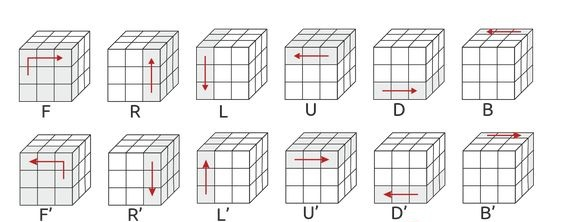
\includegraphics[width=1\linewidth]{cube_rotations}
	\caption{Способы поворота граней кубика Рубика}
	\label{fig:cube_rotations}
\end{figure}

\subsubsection{Сборка кубика Рубика}
Для сборки кубика Рубика не обязательно знать всю последовательность действий, применённую к нему, достаточно информации о цветах граней. Для сборки кубика Рубика можно применить алгоритм Джессики Фридрих \cite{bib:fridrich}.

Сборка кубика Рубика по методу Джессики Фридрих, делится на четыре этапа:
\begin{enumerate}
	\item Сборка «креста»
	\item Сборка первых двух слоёв (F2L)
	\item Ориентация кубиков верхнего слоя (OLL)
	\item Расстановка кубиков верхнего слоя (PLL)
\end{enumerate}

Каждый из этих этапов имеет конечное, относительно малое количество вариантов расположения цветов граней. Решение очередного этапа кубика Рубика состоит в определении конкретной ситуации (цветов граней), и применение соответствующей последовательности действий. Например, во время сборки OLL может возникнуть ситуация, проиллюстрированная на рис. \ref{fig:c_shape}. Её решением является следующая последовательность действий: R'U'R'FRF'UR

\begin{figure}[ht]
	\centering
	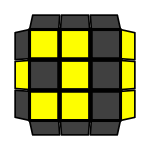
\includegraphics[width=0.25\linewidth]{c_shape}
	\caption{Ситуация, которая может возникнуть во время сборки OLL}
	\label{fig:c_shape}
\end{figure}

\subsubsection{Зеркальный кубик Рубика}
\begin{figure}[ht]
	\centering
	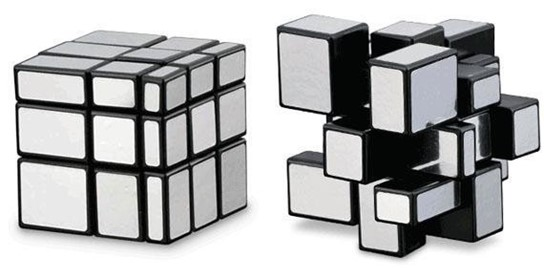
\includegraphics[width=1\linewidth]{mirrored_rubics_cube}
	\caption{Внешний вид зеркального кубика Рубика в собранном (слева) и в разрбранном (справа) состояниях}
	\label{fig:mirrored_cube}
\end{figure}

Цвет --- не единственный способ обозначать правильно собранные грани. Одной из модификаций классического кубика Рубика является зеркальный кубик Рубика. Он отличается от классической версии тем, что грани отличаются не по цвету, а по высоте каждого параллелограмма относительно центра кубика. Грань собранного кубика Рубика состоит из граней параллелограммов разного размера, но остаётся в форме квадрата; при разборке --- форма меняется. Несмотря на эти различия, зеркальная и классическая версии кубика Рубика имеют общие принципы сборки.

\subsubsection{Пропорции зеркального кубика Рубика}
Введём пропорции зеркального кубика Рубика (рисунок \ref{fig:mirrored_cube_proportions}). Пусть:
\begin{itemize}
	\item наблюдатель смотрит по направлению оси X (нормаль к грани B),
	\item строго налево от наблюдателя направлена ось Y (нормаль к грани L),
	\item сторо наверх от наблюдателя направлена ось Z (нормаль к грани U)
\end{itemize}

Тогда вдоль каждой оси последовательно отложим отрезки трёх длин:
\begin{itemize}
	\item для оси X: 17, 19, 21
	\item для оси Y: 13, 19, 25
	\item для оси Z: 9, 19, 29
\end{itemize}

Плоскости, проведённые перпендикулярно соответствующей оси на границе отрезка, отрезают трёхмерный куб размером 57x57x57, разделённый на 27 параллелограммов. 

\begin{figure}[ht]
	\centering
	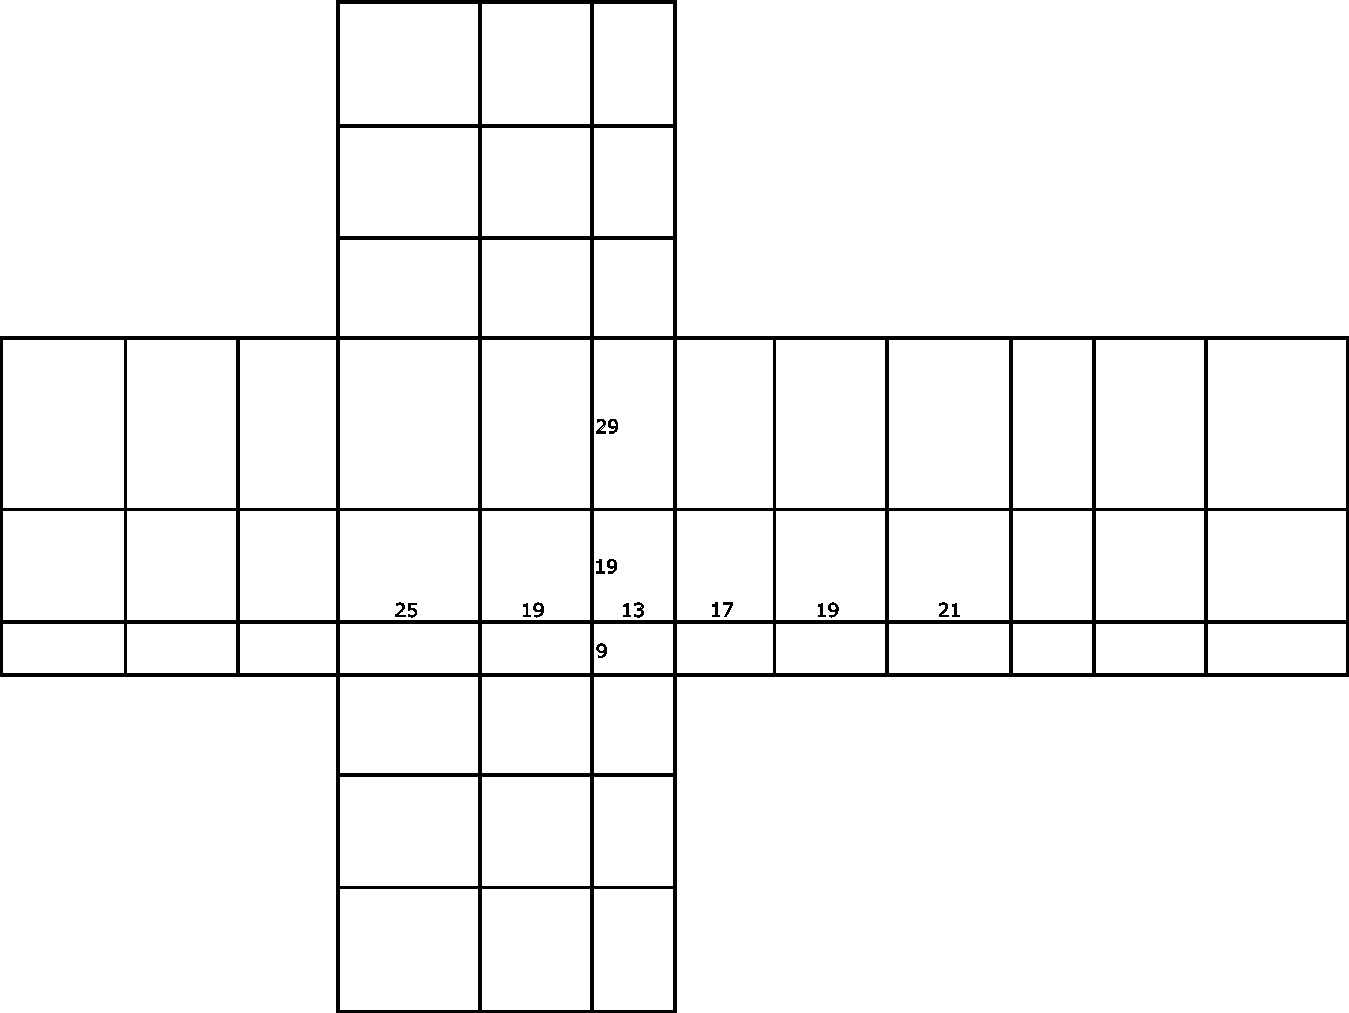
\includegraphics[width=1\linewidth]{mirrored_cube_propotions}
	\caption{Пропорции зеркального кубика Рубика}
	\label{fig:mirrored_cube_proportions}
\end{figure}

\subsection{Отрисовка сцены}
Одной из основных задач разрабатываемого програмного продукта является отрисовка зеркального кубика Рубика. Рассмотрим существующие алгоритмы удаления невидимых граней:
\begin{itemize}
	\item Алгоритм плавающего горизонта
	\item Алгоритм Варнока
	\item Алгоритм Робертса
	\item Алгоритм Вейлера-Азертона
	\item Алгоритм, Z-буфера
	\item Алгоритм, использующий список приоритетов
	\item Алгоритмы построчного сканирования
\end{itemize}

Все вышеперечисленные алгоритмы не могут привести к корректному результату, если среди объектов сцены присутствует зеркальные поверхности. Таким образом, для отрисовки зеркальных поверхностей необходимо использовать алгоритм трассировки лучей \cite{bib:computergraphics}.

\subsubsection{Алгоритм прямой трассировки лучей}
Основная идея алгоритма --- промоделировать поведение света для получения реалистичного изображения. В реальном мире, свет исходит от источника света, отражается от отражающих поверхностей и рассеивается рассеивающими поверхностями. Некоторые лучи света попадают на сетчатку глаза, которая посылает сигнал об интенсивности и цвете пришедшего луча. Алгоритм, реализующий такую модель, называется алгоритмом прямой трассировки лучей.

\subsubsection{Алгоритм обратной трассировки лучей}
\begin{figure}[ht]
	\centering
	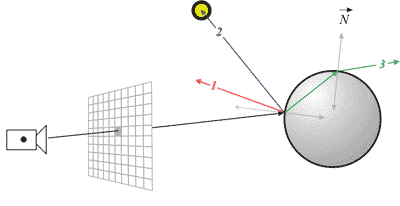
\includegraphics[width=1\linewidth]{backward_ray_trace}
	\caption{Обратная трассировка лучей}
	\label{fig:backward_ray_trace}
\end{figure}

Заметим, что нас интересуют лишь те лучи света, которые попали на сетчатку глаза. На основе этого, при моделировании подобной системы, лучи можно пускать в обратную сторону, то есть начиная от сетчатки. Теперь цвет луча при столкновении будет рассчитываться в зависимости от освещённости очередной точки попадания луча и цвета поверхности, на которую попал луч.

В качестве допущения, будем считать, что все поверхности на сцене являются непрозрачными.

\subsubsection{Описание алгоритма обратной трассировки лучей}
Алгоритму поступает следующие данные:
\begin{itemize}
	\item местополжение наблюдателя;
	\item расстояние до проецирующей плоскости;
	\item местоположение и геометрия всех объектов на сцене.
\end{itemize}

На основе этих данных, алгоритм должен окрасить сетку пикселей $n\times m$ так, чтобы при отображении её на экране, можно было распознать реалистичное изображение.

Для каждого пикселя, из камеры пускается луч в соответствующем направлении. При попадании луча в плоскость, порождается дополнительный луч, отражённый. Вектор отражения $\bar V_M$, при исходном луче $\bar V$, относительно нормали $\bar n$, при $|\bar n| = 1$ считается по следующей формуле:

\begin{equation}
	\bar V_M = \bar V - 2\cdot\bar V \cdot\bar n\cdot\bar n
	\label{eq:bounce}
\end{equation}

Цвет данной точки рассчитывается как смешение цвета поверхности и цвета, рассчитаного при попадании луча $\bar V_M$ на поверхность.

С целью упростить задачу поиска пересечения луча и поверхности, будем считать, что каждый объект сцены можно представить в виде набора из конечного числа треугольников.

\subsection{Вывод по разделу}
В аналитическом разделе был описан кубик Рубика, обозначения граней и их поворотов. Была объяснена разница между классическим кубиком Рубика и его вариацией --- зеркальным кубиком Рубика.

Так же, описана задача отрисовки трёхмерной сцены. Обозначена причина, по которой был выбран алгоритм обратной трассировки лучей в качестве способа отрисовки трёхмерной сцены.

Были установлены ограничения по содержанию сцены, а именно:
\begin{itemize}
	\item Все объекты на сцене являются непрозрачными
	\item Каждый объект сцены можно представить в виде конечного набора треугольников
\end{itemize}

